\chapter{Theoretical Foundation}\label{ch:theoretical}

\section{Machine Learning}

\begin{enumerate}
    \item Loss Function / Error Metrics
    \item Supervised --- Unsupervised / Categorization
    \item Optimization techniques: Stochastic-Batch Gradient Descent, GD Momentum, Adam
    \item Bias-Variance tradeoff / Overfitting --- Underfitting
        % FIXME: how much of optimization and bias-variance tradeoff is actually needed???
\end{enumerate}

`The prediction error of a model has three components: irreducible error, which cannot be elim-
inated regardless of the algorithm or training methods employed; bias error, due to simplifying
assumptions intended to make learning the model easier; and variance error, an estimate of how
much the model output would vary if different data were used in the training process. The aim
of training is to minimise the bias and variance errors, and therefore the objective functions
reflect these errors. The objective functions may also contain simplifying assumptions to aid
optimiza- tion, and these assumptions must not be present when assessing model
performance [59].'\citep{ashmore_assuring_2021}
See~\citep{ashmore_assuring_2021} for measures, ROC curve and cost curve
Difference in Robusteness vs Performance see~\citep{ashmore_assuring_2021} (pretty much
bias-variance tradeoff)
Robusteness: training set does not include all possible ranges of values -> ability to generalize

See~\citep{seshia_formal_2018} for mathematical notation for ML

Define generalization


The model consists of subcomponents organized in directed acyclc graph building a
pipeline~\citep{siebert_construction_2021}.
This directed acyclic graph depicts everything from processing the images to the extracted
information~\citep{siebert_construction_2021}.
\section{Deep Learning}


` One of the main differences from traditional ma- chine learning (ML) methods is that DL
automatically learns how to represent data using multiple layers of abstraction [5], [6].
In traditional ML, a significant amount of work has to be spent on “feature engineering” to
build this representation manually, but this process can now be automated to a higher degree.
Having an automated and data-driven method for learning how to represent data improves both the
performance of the model and reduces requirements for manual feature engineering work
[7], [8].'~\citep{arpteg_software_2018}

\begin{enumerate}
    \item ANN / MLP % Node, Feedforward, Backpropagation / Optimization
        \begin{itemize}
            \item Architecture $\rightarrow$ Input, Hidden, Output
            \item Feedforward
            \item Optimization $\rightarrow$ Backpropagation, SGD, ADAM, \ldots
        \end{itemize}
    \item Regularization: L0,L1,L2, Dropout, Dropconnect
    \item important architectures
        \begin{itemize}
            \item CNN % layers --- convolutional, max-pooling
            \item RNN % recurrent layer
            \item Specific foundation architectures for relevant approaches
        \end{itemize}
    \item transfer learning: reuse parameters from pretrained models\\


For reusability: see~\citep{ashmore_assuring_2021}: `Convolutional neural networks (CNN) are
particularly suited for partial model transfer [59] since the convolutional layers encode
features in the input space, whilst the fully connected layers encode reasoning based on those
features.'


\end{enumerate}

\textbf{Deep Learning in Character Recognition Considering Pattern Invariance
Constraints}~\citep{oyedotun_deep_2015}
Deep Learning: neural network architecture of more than a single hidden layer as opposed to shallow networks
Features of deep networks: distributed representation of knowledge at each hidden layer, distinct
features are extracted by units or neurons in each hidden layer
several units can be active concurrently
Each layer extracts moredefined/advanced features $\rightarrow$ hierarchical representation of
features

Common problems with training deep learning
\begin{itemize}
    \item saturating units
    \item vanishing gradients
    \item over-fitting \& underfitting
\end{itemize}

Classification of deep learning architectures
\begin{itemize}
    \item Generative Architectures:\\
        not deterministic of class patterns that input belong to $\rightarrow$ sample joint
        statistical distribution of data\\
        unsupervised learning: greedy layer-wise pre-training\\
        Use auto encoders (generative) when a lot unlabelled but not a lot labelled data
        $\rightarrow$ generatively train network and then fine tune with labelled
    \item Discriminative Architectures:\\
        required to be deterministic of correlation of input data to the classes of patterns therein\\
        supervised learning
    \item Hybrid\\
        combination of discriminative and generative\\
        generally pre-trained and discriminately fine-tuned for deterministic purposes
\end{itemize}

\subsection*{Transfer Learning}
Factors in Finetuning Deep Model for Object Detection with Long-tail
Distribution~\citep{ouyang_factors_2016}
finetuning: appraoch dat initializes model parameters for target task from parameters pretrained on
another related task

\subsection*{Convolutional Neural Network}
\textbf{Comparative analysis of deep learning image detection
algorithms}~\citep{srivastava_comparative_2021}
These layers apply filters to extract patterns from images. The filter moves over the image to generates the output. Different filters recognize different patterns. Initial layers have filters to recognize simple patterns. They become more complex through the layers over time as follows:

\textbf{Review of Deep Learning Algorithms and Architectures}~\citep{shrestha_review_2019}
Def Neural Network:
\begin{itemize}
    \item Machine Learning technique that consists of processing units organized in input,
        hidden and output layers
    \item the nodes or units in each layer are connected to nodes in adjacent layers
    \item each connection has weight value
    \item inputs are multiplied by weight and summed up at each unit
    \item the sum is used with an activation function (e.g. ReLU, Sigmoid, Tanh, SoftPlus)
\end{itemize}

\section{Optical Character Recognition}

\textbf{Deep Learning based OCR}~\citep{zhao_improving_2020}
What is OCR:\ process of converting images of typed, handwritten or printed text into machine-encoded one
includes two sub frameworks: text detection and text recognition (based on position coordinates)
\textbf{End-To-End also possible}
Process can include image processing!!!

Text Recognition in the Wild: A Survey~\citep{chen_text_2021}
\begin{itemize}
    \item various stages of \ac{OCR}:
        \begin{itemize}
            \item text localization: localize text components, group into candidate text regions with
                as little background as possible, DNN
            \item text verification: verify text candidate regions as text or non-text,
                filter false-positives, CNN
            \item text detection: determine whether text is present using localization and verification
                procedures, basis for end-to-end, can be regression or segmentation based
            \item text segmentation: most challenging, includes text line (splitting a region of multiple
                text lines into subregion of single text lines) and character segmentation (separating
                text instance into single characters, typically used in earlier approaches)
            \item text recognition: translates cropped text instance image into target string sequence,
                basis for end-to-end, DL encoder-decoder frameworks
            \item end-to-end-system: given scene text image $\rightarrow$ convert all text regions into
                target string sequences, includes detectoin, recognition and postprocessing, can be
                seen as indipendent subproblems but also joint by sharing information
        \end{itemize}
    \item text enhancement: recover degraded text, improve text resolution, remove distortions,
        remove background $\rightarrow$ reduce difficulty of recognition
\end{itemize}
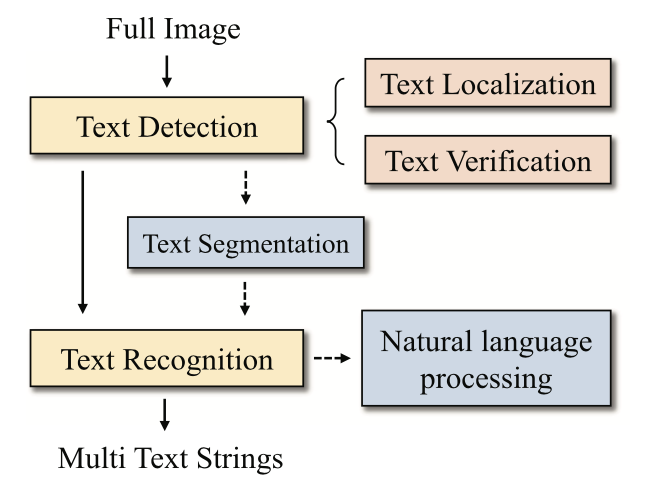
\includegraphics{img/OCR-Basics.png}


\textbf{no source}
grid: divides image into parts $\rightarrow$ each part has own bounding boxes
bounding boxes:~regressor for box, each bounding box is assigned an anchor box (respective to grid cell)
anchor boxes:~default `shape' for bounding box

bounding boxes different stages of convolution / 2-d size $\rightarrow$ different object size to detect

\subsection*{Text detection}
subfield of object detection (e.g. YOLOv4 can be used for text)

Detect position coordinates containing text in input image
Text detection more challenging

Two object detection methods --- CNN-based
\begin{itemize}
    \item Region-based \\
        views detection problem as classification problem\\
        CNN to extract deep features of proposals by selective search $\rightarrow$  Use SVM to
            classify with features\\
        e.g. R-CNN
    \item  single `look'
        extract feature maps on entire image\\
        directly regress bounding boxes on feature maps\\
        e.g. YOLO --- You Only Look Once, SSD --- Single Shot Detection
\end{itemize}
Non CNN-based: DETR

\subsubsection*{Comparison Object Detection basic algos}
\textbf{Comparative analysis of deep learning image detection
algorithms}~\citep{srivastava_comparative_2021}
YOLO-V3 outperforms SSD and Faster R-CNN

VGG-16 widely used feature generating architecture

\subsubsection*{Faster-RCNN}
A deeper look at how Faster-RCNN works~\citep{goswami_deeper_2018}
composed of 3 neural nets:
\begin{itemize}
    \item Feature Network: pre-trained image classification netork $\rightarrow$ generate good features
    \item Region Proposal Network:
        \begin{itemize}
            \item NN with 3 conv layers
            \item one layer splits up network to: classification and bounding box regression
            \item bounding box regression $\rightarrow$ bounding boxes are region of interes (ROI)
                that might contain an object
        \end{itemize}
    \item Detection Network: take input from previous nets, generate final class and bounding box,
        4 fully connected, 2 stacked common layers shared by classification and bounding box regression
        layer \end{itemize}

\textbf{Deep Learning in Character Recognition Considering Pattern Invariance
Constraints}~\citep{oyedotun_deep_2015}
Neural networks can learn features of task on which they are designed and trained
Neural networks better than other approaches (e.g.\ template matching, syntactic analysis)
$\rightarrow$ NNs can learn and adapt to moderate variations (e.g.\ translation, rotation, scaling,
noisy patterns)

\subsection*{Text Recognition}
Recognize text based on position coordinates

character based or word based

Visual attention models for scene text recognition~\citep{ghosh_visual_2017}
Divided into word detection (generate bounding boxes) and word recognition
word recognition can be divided into dictionary-based methods and unconstrained methods

\subsection*{End-To-End}
